\begin{frame}{General Updates}
    \begin{itemize}
        \item Still waiting on test dataset
        \item Resolved some issues during model training
        \item Got some interesting results!
    \end{itemize}    
\end{frame}


% Slides for 2024-08-13
% To create a slide, use the following:
% \begin{frame}{TITLE}
%     BODY
% \end{frame}

% To create a slide with a bullet list, use the following:
% \begin{frame}{TITLE}
%     \begin{itemize}
%         \item ITEM 1
%         \item ITEM 2
%     \end{itemize}    
% \end{frame}

% To create a slide with numbered list, use the following:
% \begin{frame}{TITLE}
%     \begin{enumerate}
%         \item ITEM 1
%         \item ITEM 2
%     \end{enumerate}
% \end{frame}

% To create a slide with a graphic:
% 1. Add the graphic to this folder (named picture.png)
% 2. Use the following:
% \begin{frame}{TITLE}
%     \centering
%     \includegraphics[height=0.7\textheight,width=0.7\textwidth,keepaspectratio]{picture.png}
% \end{frame}

% To create a slide with two columns, use the following:
% \begin{frame}{TITLE}
%     \begin{columns}
%         \begin{column}{0.5\textwidth}
%             COLUMN 1 BODY
%         \end{column}
%         \begin{column}{0.5\textwidth}
%             COLUMN 2 BODY
%         \end{column}
%     \end{columns}
% \end{frame}

\begin{frame}
    \frametitle{Desktop Application}

    \begin{figure}
        \centering
        \begin{minipage}{0.48\textwidth}
            \centering
            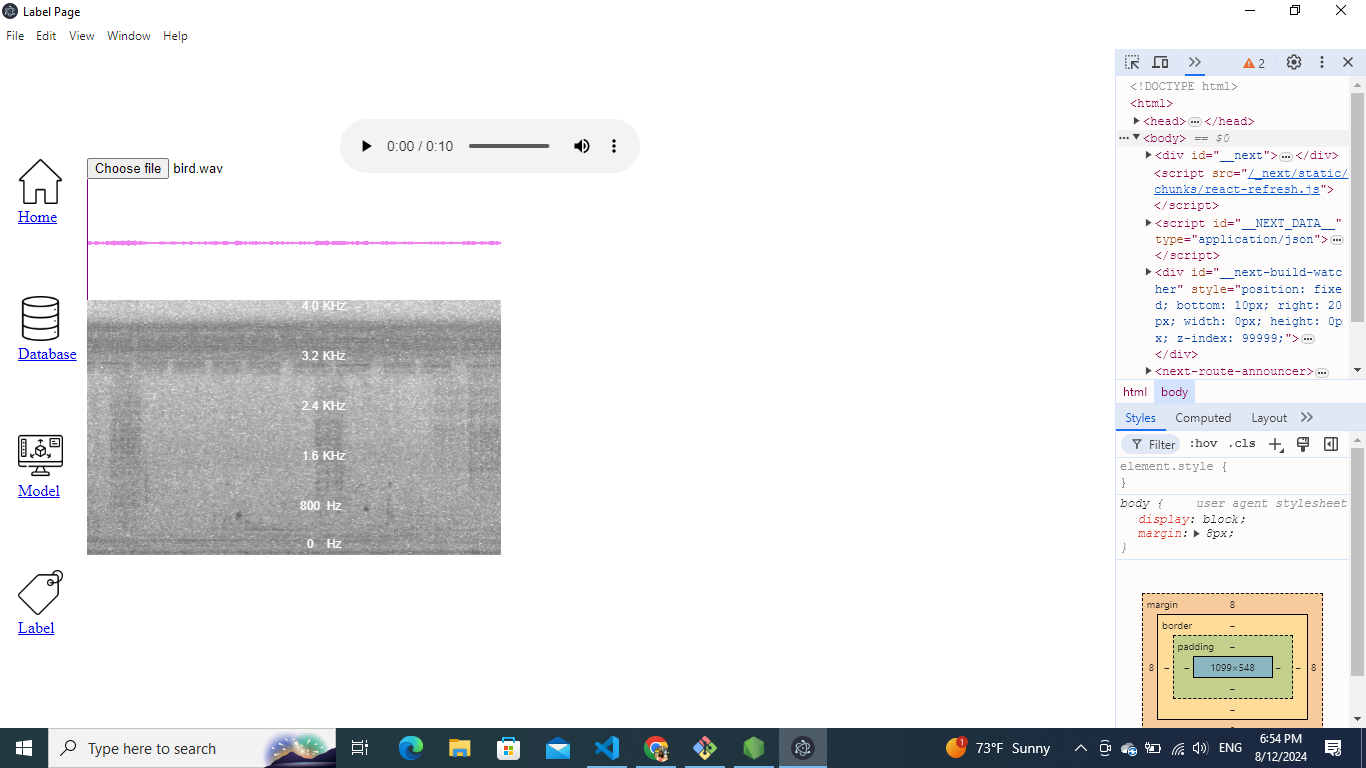
\includegraphics[width=\textwidth]{label.png}
            \caption{Label Page}
        \end{minipage}
        \hfill
        \begin{minipage}{0.48\textwidth}
            \centering
            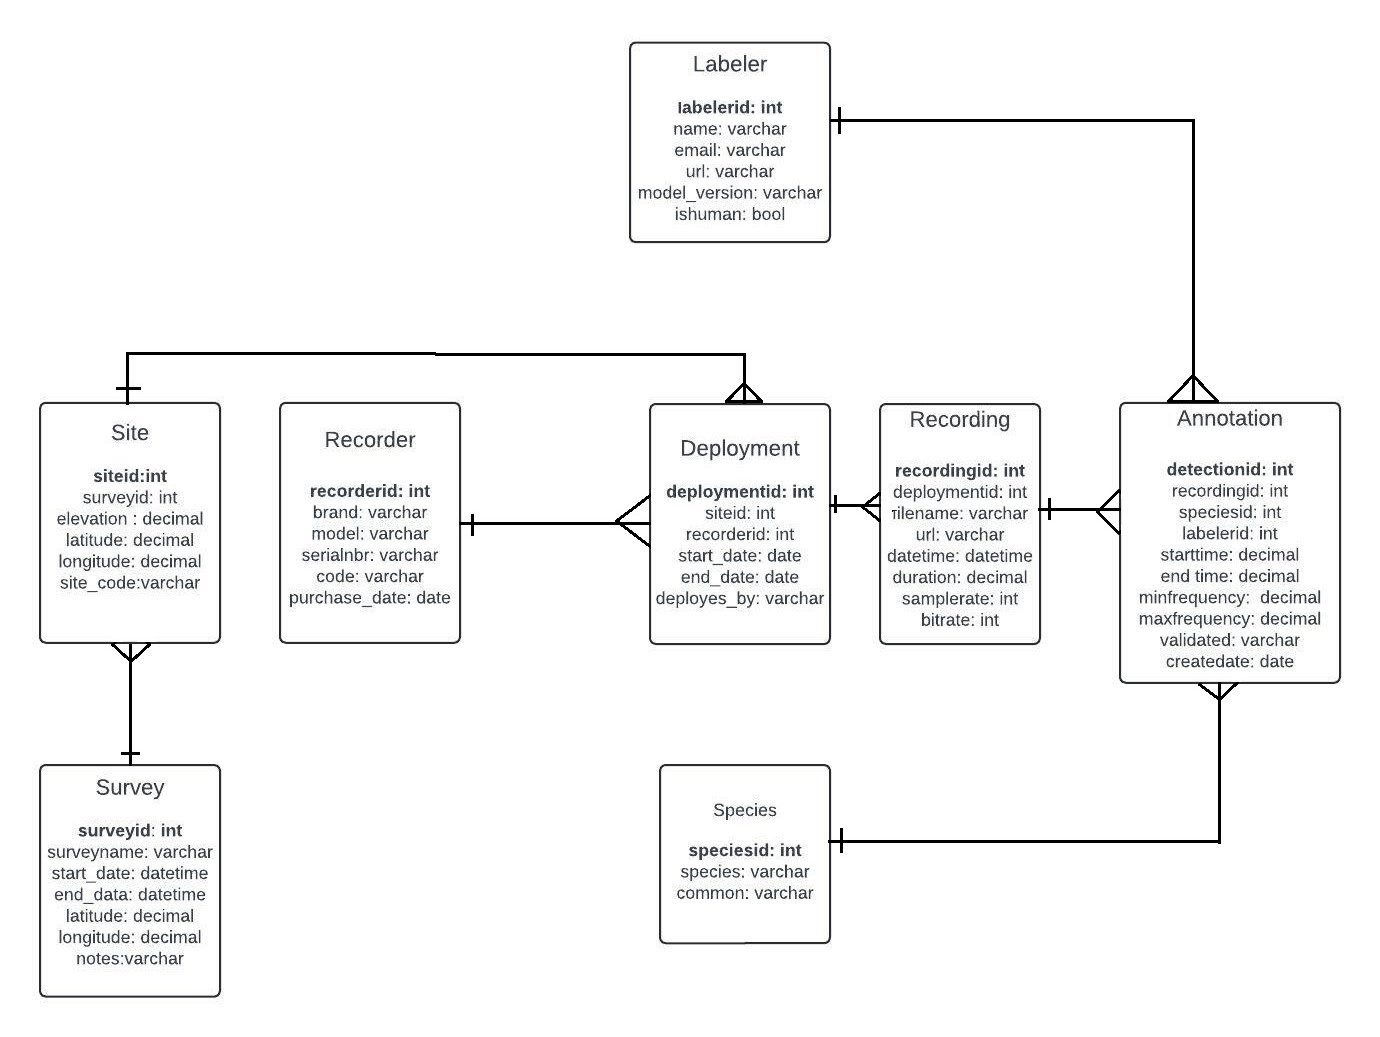
\includegraphics[width=\textwidth]{database.jpg}
            \caption{Database Schema}
        \end{minipage}
    \end{figure}

\end{frame}


\begin{frame}{LEAF Progress}
    \centering
    After 20 Epochs
    \break
    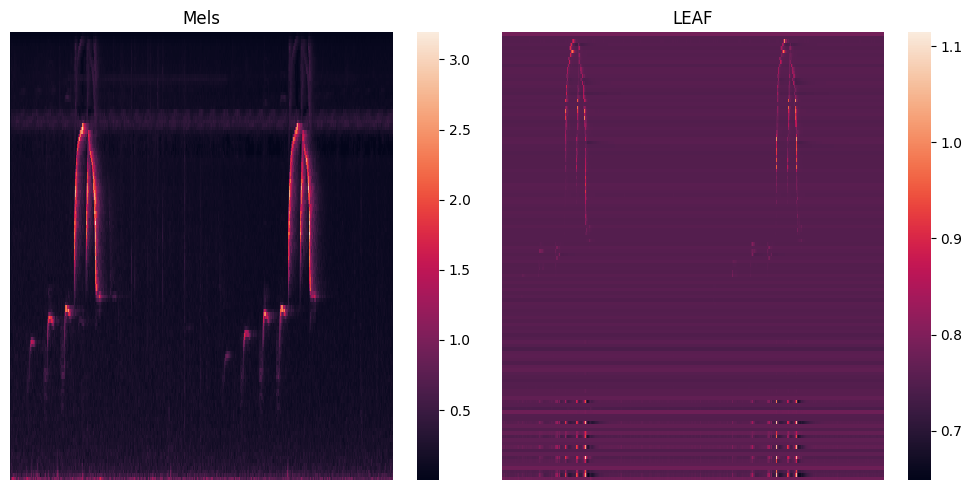
\includegraphics[height=0.7\textheight,width=0.7\textwidth,keepaspectratio]{images/LEAF_20.png}
\end{frame}

\begin{frame}{LEAF Progress}
    \centering
    After 80 Epochs
    \break
    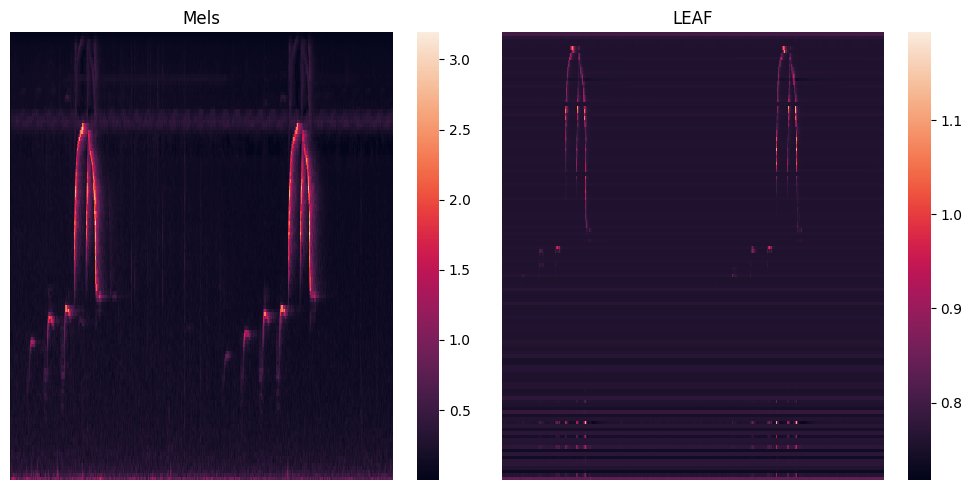
\includegraphics[height=0.7\textheight,width=0.7\textwidth,keepaspectratio]{images/LEAF_80.png}
\end{frame}

\begin{frame}{BirdAVES Model Training}
    \begin{columns}
        \begin{column}{0.5\textwidth}
        \begin{itemize}
        \item Issues with training BirdAVES large model
        \item expermenting with DA and learning rate
        \item Model training is still ongoing
        \item Next step: test model
        \end{itemize}
    \end{column}
    \begin{column}{0.5\textwidth}
        \centering
        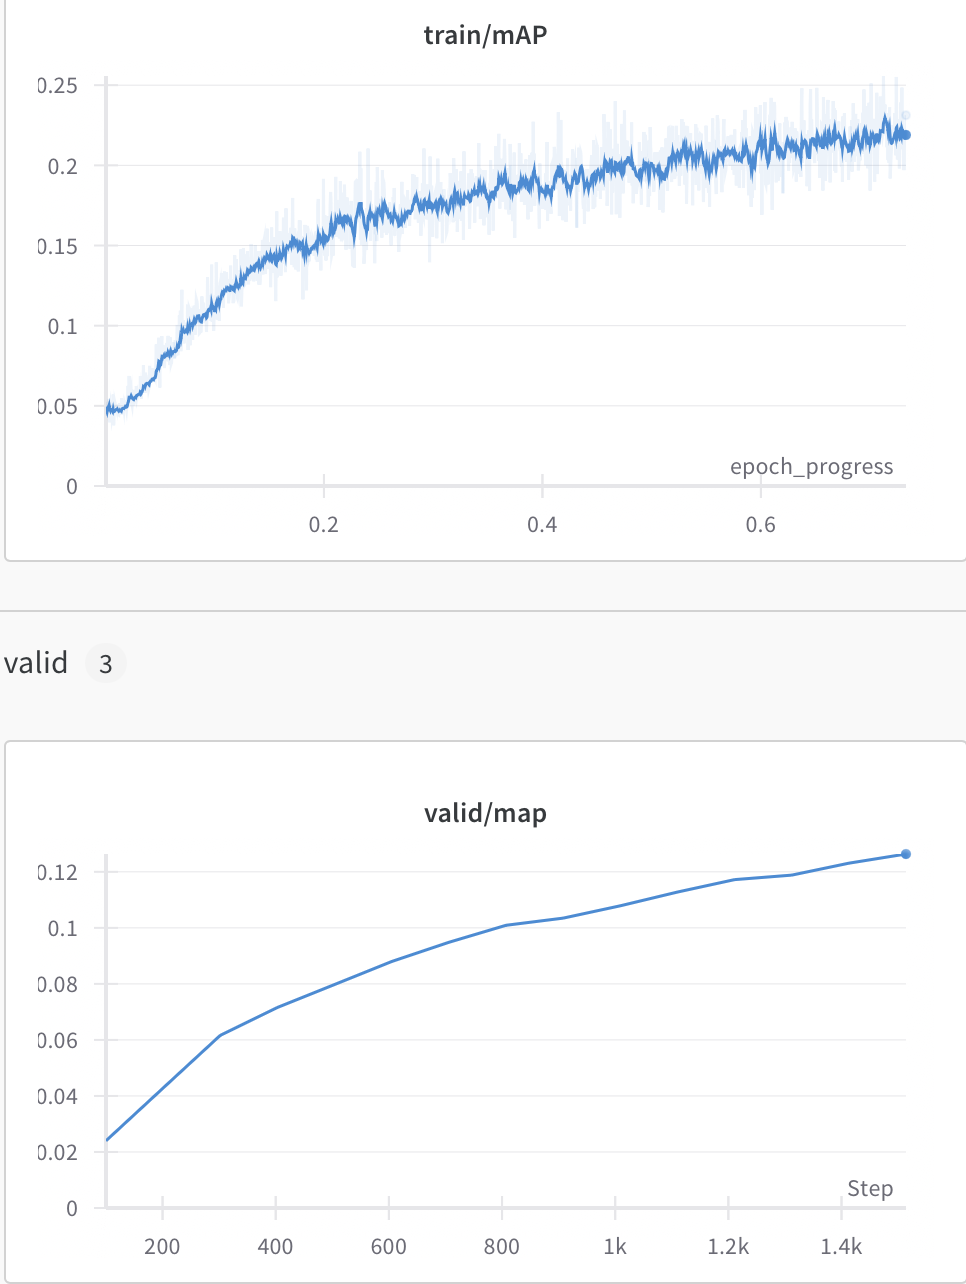
\includegraphics[height=0.85\textheight,width=1\textwidth,keepaspectratio]{images/BirdAVES_cmap.png} 
    \end{column}   
    \end{columns}
\end{frame}

\begin{frame}{Analysis: Acoustic Spectrum Transformer}
    \begin{columns}
        \begin{column}{0.5\textwidth}
        \begin{itemize}
        \item LR: 4e-5, 1e-5, 5e-6
        \item Epoch: less than 2 (validation decreases after ~35K steps)
        \item precision 0.643
        \item recall 0.53
        \item f1 0.55
        \item next steps: cross compare with a CNN model (ResNet50?)
        \end{itemize}
    \end{column}
    \begin{column}{0.5\textwidth}
        \centering
        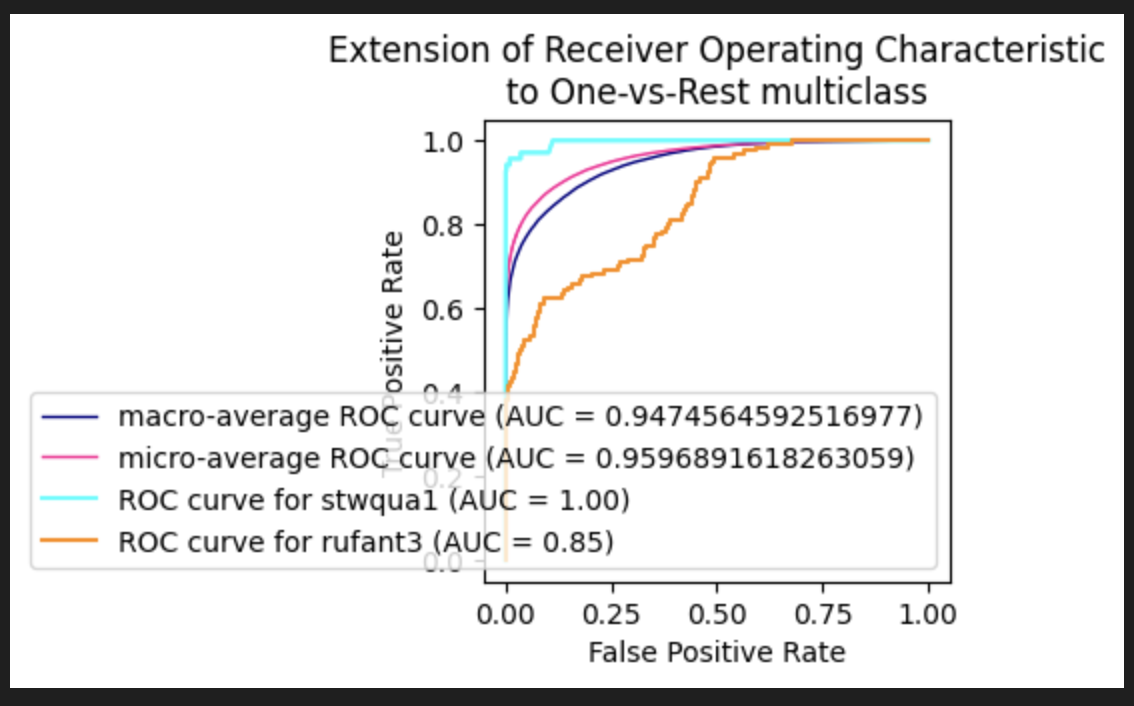
\includegraphics[height=0.85\textheight,width=1\textwidth,keepaspectratio]{images/ast_auc.png} 
    \end{column}   
    \end{columns}
\end{frame}